% Options for packages loaded elsewhere
\PassOptionsToPackage{unicode}{hyperref}
\PassOptionsToPackage{hyphens}{url}
%
\documentclass[
]{article}
\usepackage{amsmath,amssymb}
\usepackage{lmodern}
\usepackage{iftex}
\ifPDFTeX
  \usepackage[T1]{fontenc}
  \usepackage[utf8]{inputenc}
  \usepackage{textcomp} % provide euro and other symbols
\else % if luatex or xetex
  \usepackage{unicode-math}
  \defaultfontfeatures{Scale=MatchLowercase}
  \defaultfontfeatures[\rmfamily]{Ligatures=TeX,Scale=1}
\fi
% Use upquote if available, for straight quotes in verbatim environments
\IfFileExists{upquote.sty}{\usepackage{upquote}}{}
\IfFileExists{microtype.sty}{% use microtype if available
  \usepackage[]{microtype}
  \UseMicrotypeSet[protrusion]{basicmath} % disable protrusion for tt fonts
}{}
\makeatletter
\@ifundefined{KOMAClassName}{% if non-KOMA class
  \IfFileExists{parskip.sty}{%
    \usepackage{parskip}
  }{% else
    \setlength{\parindent}{0pt}
    \setlength{\parskip}{6pt plus 2pt minus 1pt}}
}{% if KOMA class
  \KOMAoptions{parskip=half}}
\makeatother
\usepackage{xcolor}
\IfFileExists{xurl.sty}{\usepackage{xurl}}{} % add URL line breaks if available
\IfFileExists{bookmark.sty}{\usepackage{bookmark}}{\usepackage{hyperref}}
\hypersetup{
  hidelinks,
  pdfcreator={LaTeX via pandoc}}
\urlstyle{same} % disable monospaced font for URLs
\usepackage[margin=1in]{geometry}
\usepackage{graphicx}
\makeatletter
\def\maxwidth{\ifdim\Gin@nat@width>\linewidth\linewidth\else\Gin@nat@width\fi}
\def\maxheight{\ifdim\Gin@nat@height>\textheight\textheight\else\Gin@nat@height\fi}
\makeatother
% Scale images if necessary, so that they will not overflow the page
% margins by default, and it is still possible to overwrite the defaults
% using explicit options in \includegraphics[width, height, ...]{}
\setkeys{Gin}{width=\maxwidth,height=\maxheight,keepaspectratio}
% Set default figure placement to htbp
\makeatletter
\def\fps@figure{htbp}
\makeatother
\setlength{\emergencystretch}{3em} % prevent overfull lines
\providecommand{\tightlist}{%
  \setlength{\itemsep}{0pt}\setlength{\parskip}{0pt}}
\setcounter{secnumdepth}{-\maxdimen} % remove section numbering
\usepackage{booktabs}
\usepackage{longtable}
\usepackage{array}
\usepackage{multirow}
\usepackage{wrapfig}
\usepackage{float}
\usepackage{colortbl}
\usepackage{pdflscape}
\usepackage{tabu}
\usepackage{threeparttable}
\usepackage{threeparttablex}
\usepackage[normalem]{ulem}
\usepackage{makecell}
\usepackage{xcolor}
\ifLuaTeX
  \usepackage{selnolig}  % disable illegal ligatures
\fi

\author{}
\date{\vspace{-2.5em}}

\begin{document}

\hypertarget{results}{%
\section{Results}\label{results}}

NEW TO PASCAL: The controlled drills part is a first draft. The specific
drills section is NOT done, and is only a few components, but it gives
an idea of the plots I am gonna use to tell ``a story''. I have yet to
actually model if it can get predicted, but it will come soon.

\hypertarget{controlled-drills}{%
\subsection{Controlled Drills}\label{controlled-drills}}

The locomotion validation test was done using a percentage-agreement
test between the label chosen for the drill (linear or non-linear
locomotion) and the prediction from the no-intensity FMP locomotions
(four categories, see figure @ref(fig:flowchartAgreement)). Table
@ref(tab:agreement) shows the overall agreement for the controlled
drills. A very good agreement can be seen for the lower velocity linear
locomotions and high velocity non-linear locomotion. However, a decrease
in agreement is occuring when the linear velocity increases and is also
lower for the lower velocity non-linear compared to the higher
velocities.

\begin{verbatim}
## -- Attaching packages --------------------------------------- tidyverse 1.3.1 --
\end{verbatim}

\begin{verbatim}
## v ggplot2 3.3.5     v purrr   0.3.4
## v tibble  3.1.6     v dplyr   1.0.8
## v tidyr   1.2.0     v stringr 1.4.0
## v readr   2.1.2     v forcats 0.5.1
\end{verbatim}

\begin{verbatim}
## -- Conflicts ------------------------------------------ tidyverse_conflicts() --
## x dplyr::filter() masks stats::filter()
## x dplyr::lag()    masks stats::lag()
\end{verbatim}

\begin{verbatim}
## 
## Attaching package: 'kableExtra'
\end{verbatim}

\begin{verbatim}
## The following object is masked from 'package:dplyr':
## 
##     group_rows
\end{verbatim}

\begin{table}[H]

\caption{\label{tab:agreement}Table of the agreement between FMP locomotion and performed drills.}
\centering
\begin{tabular}[t]{c|c|c|c}
\hline
Drill & Velocity [km/h] & Total elapsed time [s] & Agreement [\%]\\
\hline
\cellcolor{gray!6}{Walking} & \cellcolor{gray!6}{5.4} & \cellcolor{gray!6}{3655} & \cellcolor{gray!6}{99.21}\\
\hline
Running & 12 & 2016 & 95.49\\
\hline
\cellcolor{gray!6}{Running} & \cellcolor{gray!6}{18} & \cellcolor{gray!6}{1386} & \cellcolor{gray!6}{88.31}\\
\hline
Running & 19.6 & 558 & 81.00\\
\hline
\cellcolor{gray!6}{Running} & \cellcolor{gray!6}{21.6} & \cellcolor{gray!6}{558} & \cellcolor{gray!6}{74.01}\\
\hline
Dynamic & 3 sec per cone & 1273 & 75.73\\
\hline
\cellcolor{gray!6}{Dynamic} & \cellcolor{gray!6}{All out (full circle)} & \cellcolor{gray!6}{706} & \cellcolor{gray!6}{98.30}\\
\hline
Dynamic & All out (half circle) & 347 & 97.98\\
\hline
\end{tabular}
\end{table}

Figure @ref(fig:NIU2Run15) is an example of where the
mis-classifications occur for the linear drill moving at 18 km/h while
also showing the difference between the players, some are classified
perfectly, some are not. When it miss classifies linear locomotion it is
always non-linear locomotion that is classified. Figure
@ref(fig:NIU3mediumDynamic2) illustrated a non-linear drill with medium
velocity of three different subjects performing the same drill. This
shows vastly different movement patterns according to FMP which results
in a lower percentage-agreement. These FMP predictions is not
necessarily wrong as the the overall drill labelling does not take into
account small variatons in the athletes movement pattern, though they
give an indication of where FMP can be improved.

\begin{figure}

{\centering 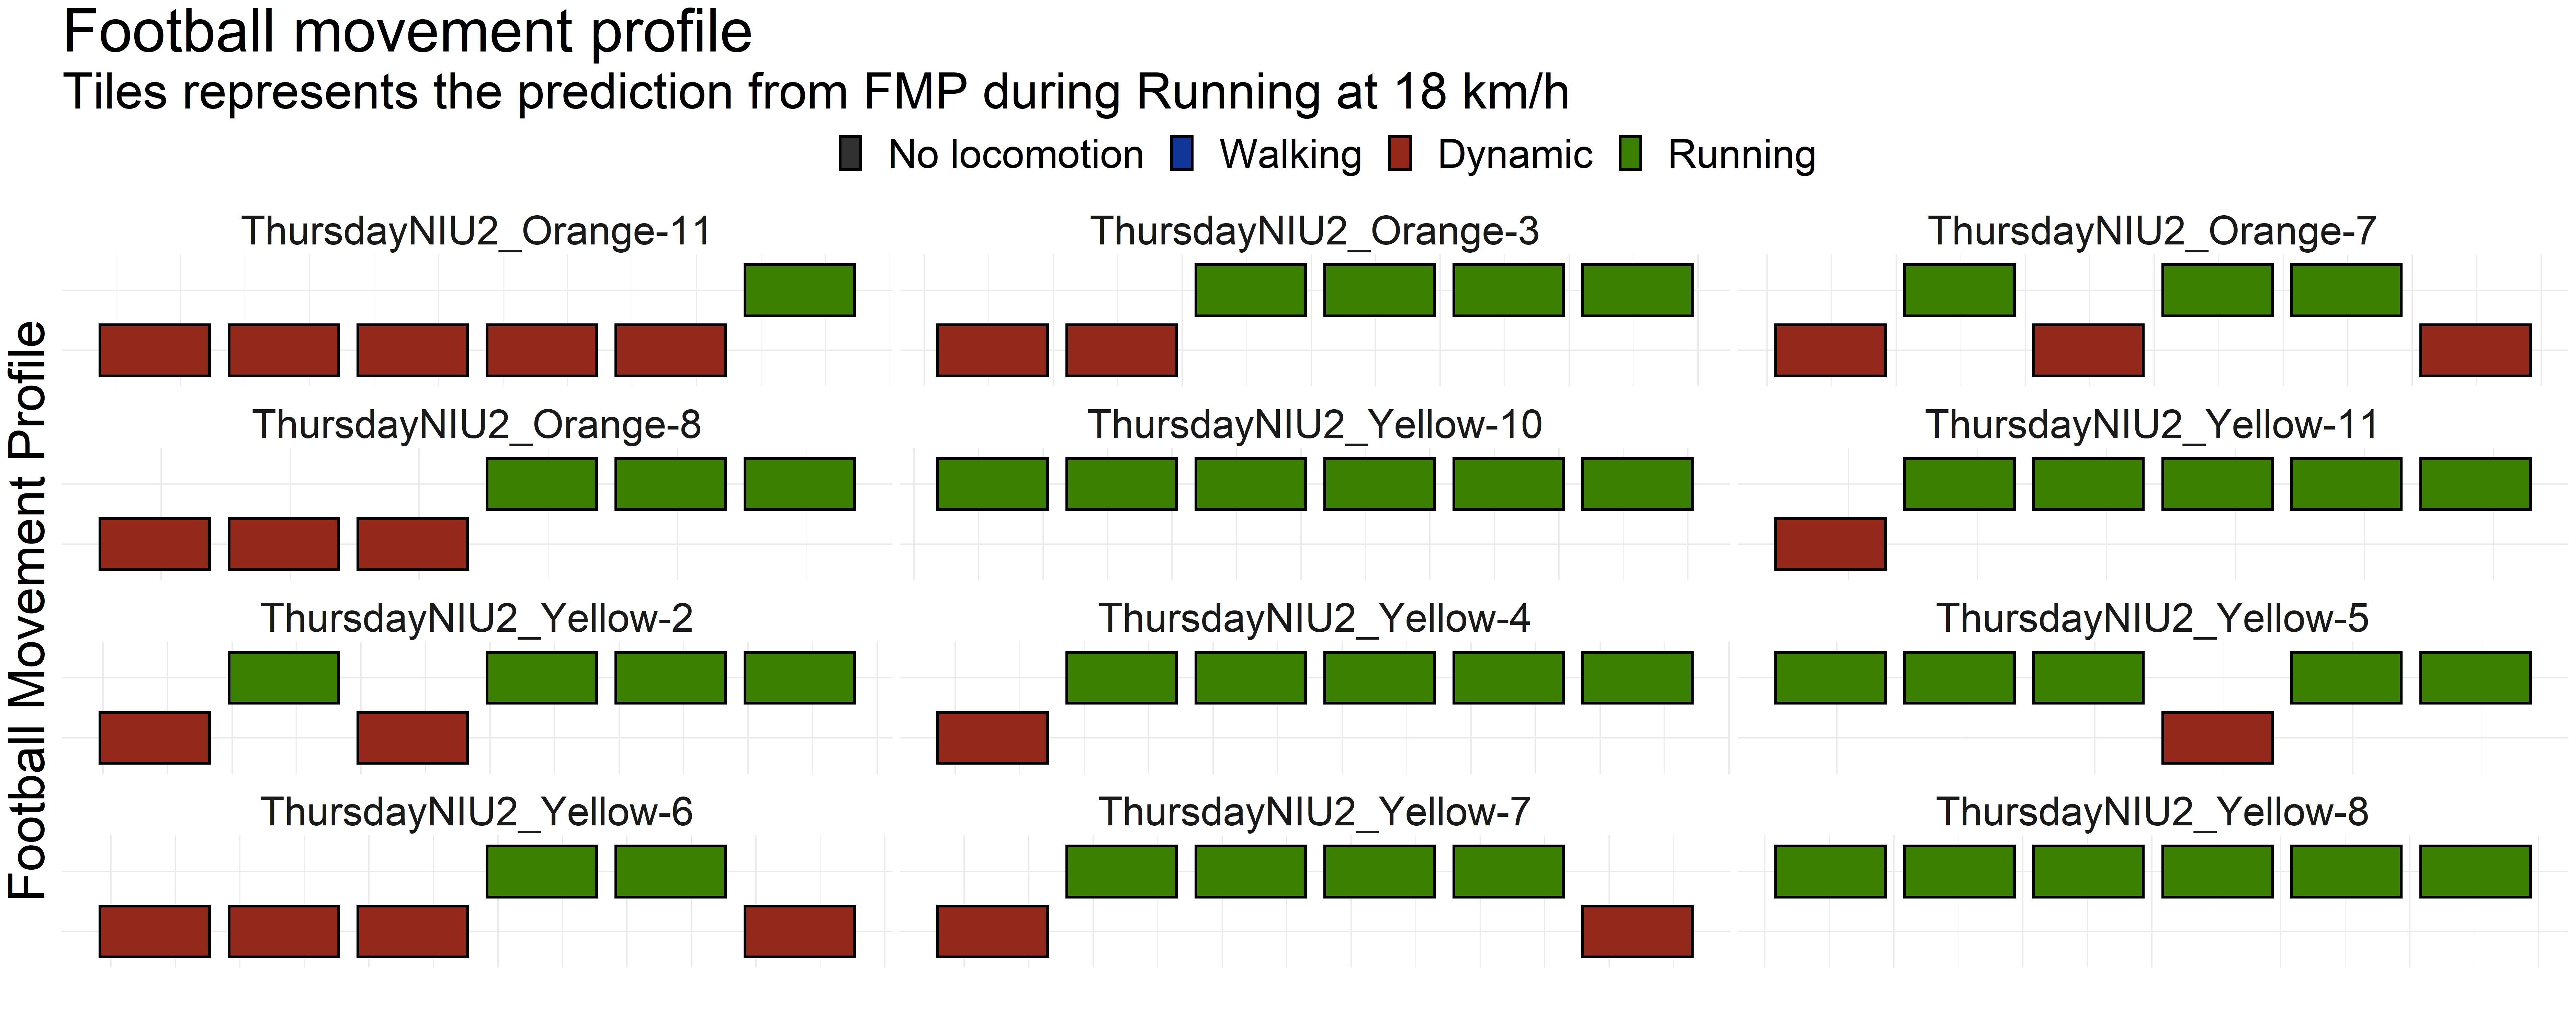
\includegraphics[width=1\linewidth]{img/Thursday_NIU2_Run15_1} 

}

\caption{FMP predictions for linear locomotion at 18 km/h for some of the players. x-axis is time, y-axis is the FMP}\label{fig:NIU2Run15}
\end{figure}

\begin{figure}

{\centering 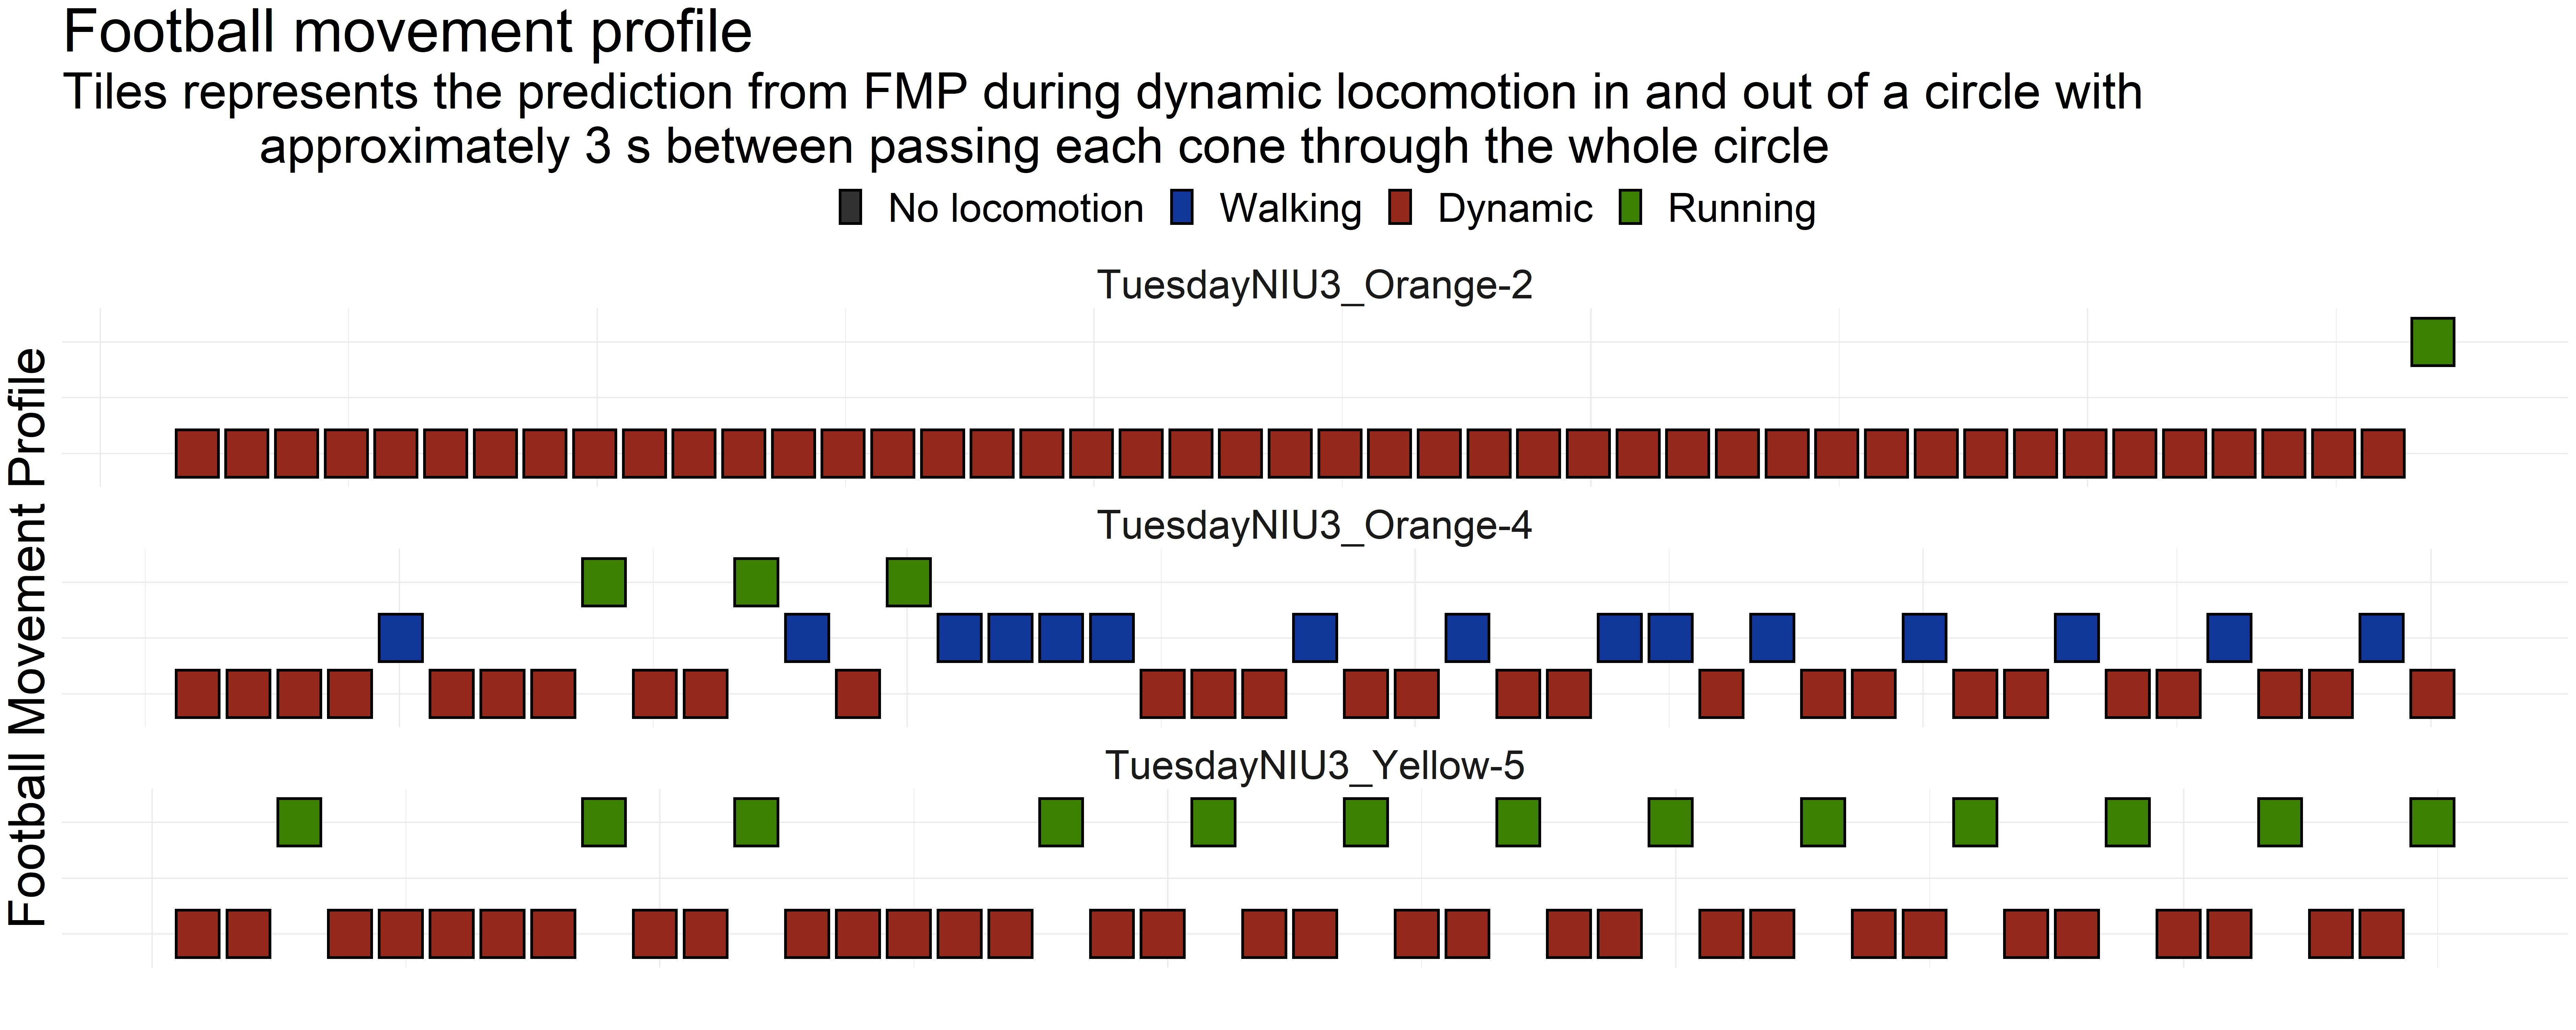
\includegraphics[width=1\linewidth]{img/Tuesday_NIU3_mediumDynamic2_3} 

}

\caption{FMP predictions for non-linear locomotion at medium intensity for some of the players. x-axis is time, y-axis is the FMP}\label{fig:NIU3mediumDynamic2}
\end{figure}

\hypertarget{specific-drills}{%
\subsection{Specific Drills}\label{specific-drills}}

Four different drills were executed. Figure @ref(fig:distribution) shows
small variations in the FMP between the drills. The big drill has more
RHI and VLI than the others, and 22\_x\_12\_b has more DMI relative to
VLI compared to the other drills. Furthermore, we can see that the
relative difference between each iteration of the same drill shows low
variation as the internal FMP distribution does not change much.

The bigram distribution (see figure @ref(fig:bigram)) illustrates that
there are noticeable differences in the movements patterns between the
drill types. Especially between the big drill where ``VLI VLI'' is the
dominant bigram, and ``DMI DMI'' is the dominant for the 22x12 drills
which corresponds with the distribution pattern from figure
@ref(fig:distribution).

\begin{figure}

{\centering 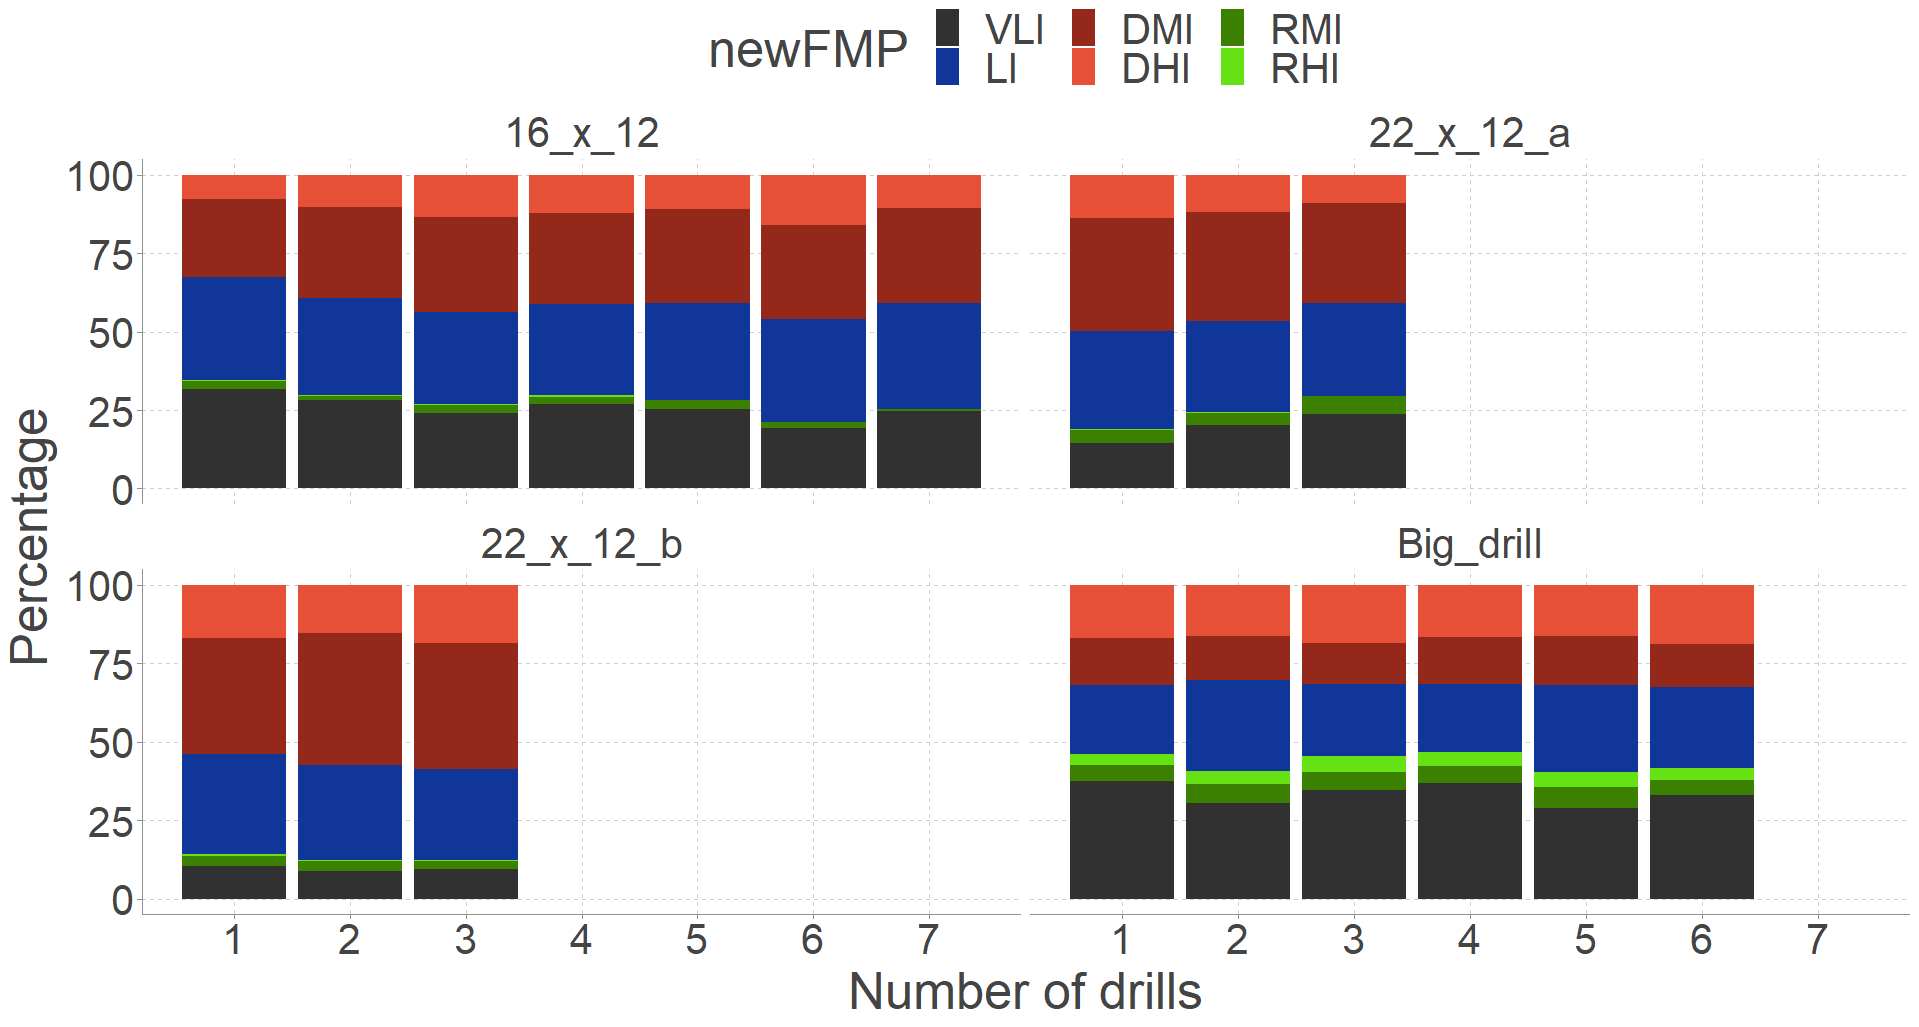
\includegraphics[width=1\linewidth]{img/distributionStackedPlot} 

}

\caption{FMP distribution for each controlled drill for each iteration. X-axis shows each iteration of the drill, Y-axis illustrated the percentage distribution.}\label{fig:distribution}
\end{figure}

\begin{figure}

{\centering 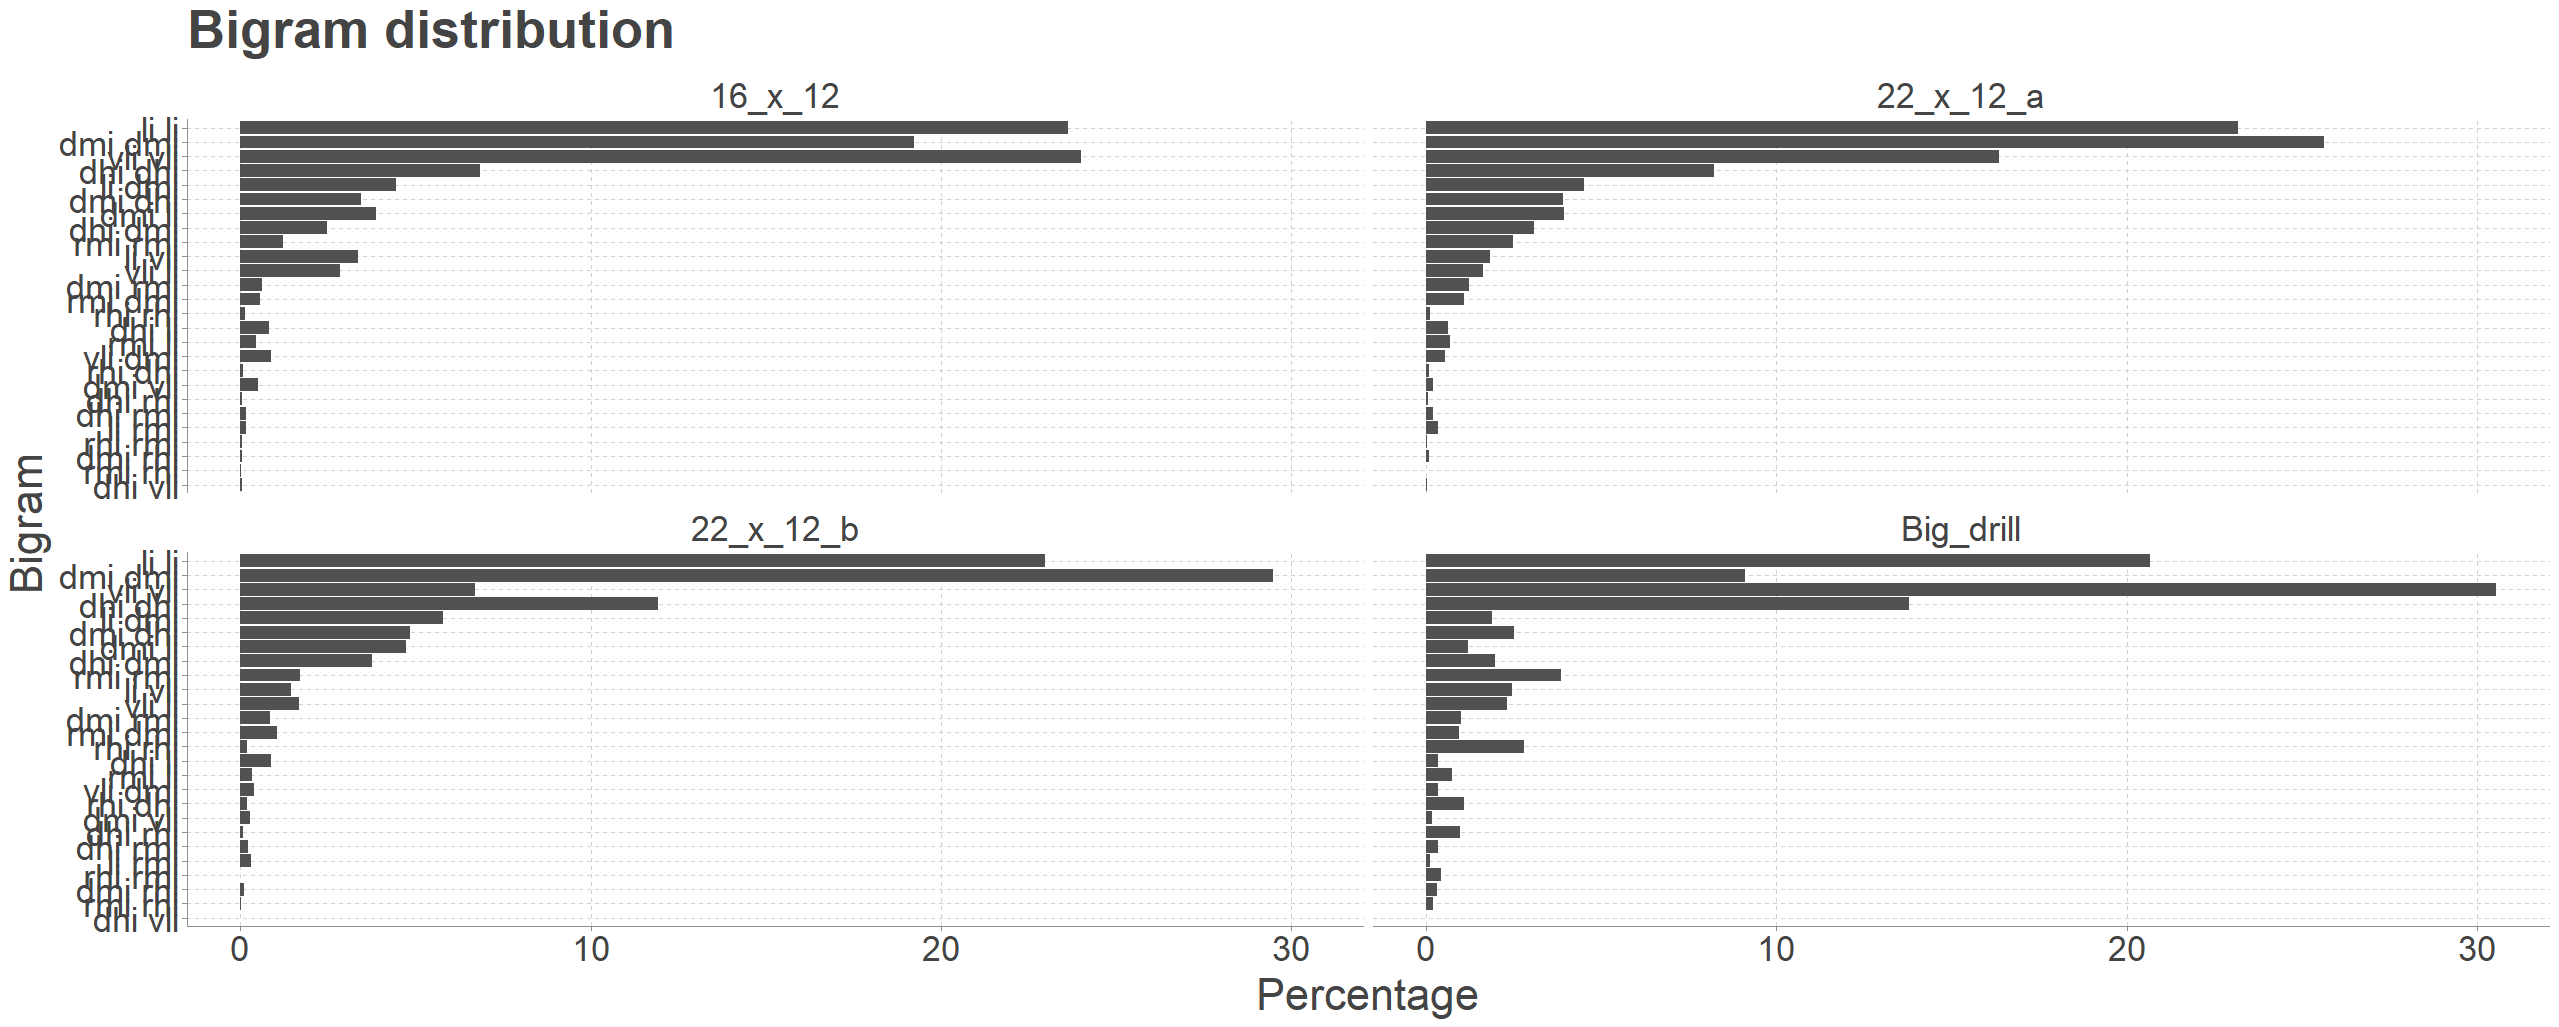
\includegraphics[width=1\linewidth]{img/bigramDistribution} 

}

\caption{FMP bigram distribution for each controlled drill. X-axis illustrated the percentage distribution and y-axis shows the FMP bigram.}\label{fig:bigram}
\end{figure}

Futhermore, the bigram also makes it possible to create a network plot
(see figure @ref(fig:network)) that illustrates the relative transition
probability (the hue of the arrows) between each category. For an
example, transition to VLI is much more frequent for the Big Drill than
the other three drills, and we also see more frequent transition from
DHI to RHI for the big drill relative to the others drills.

\begin{figure}

{\centering 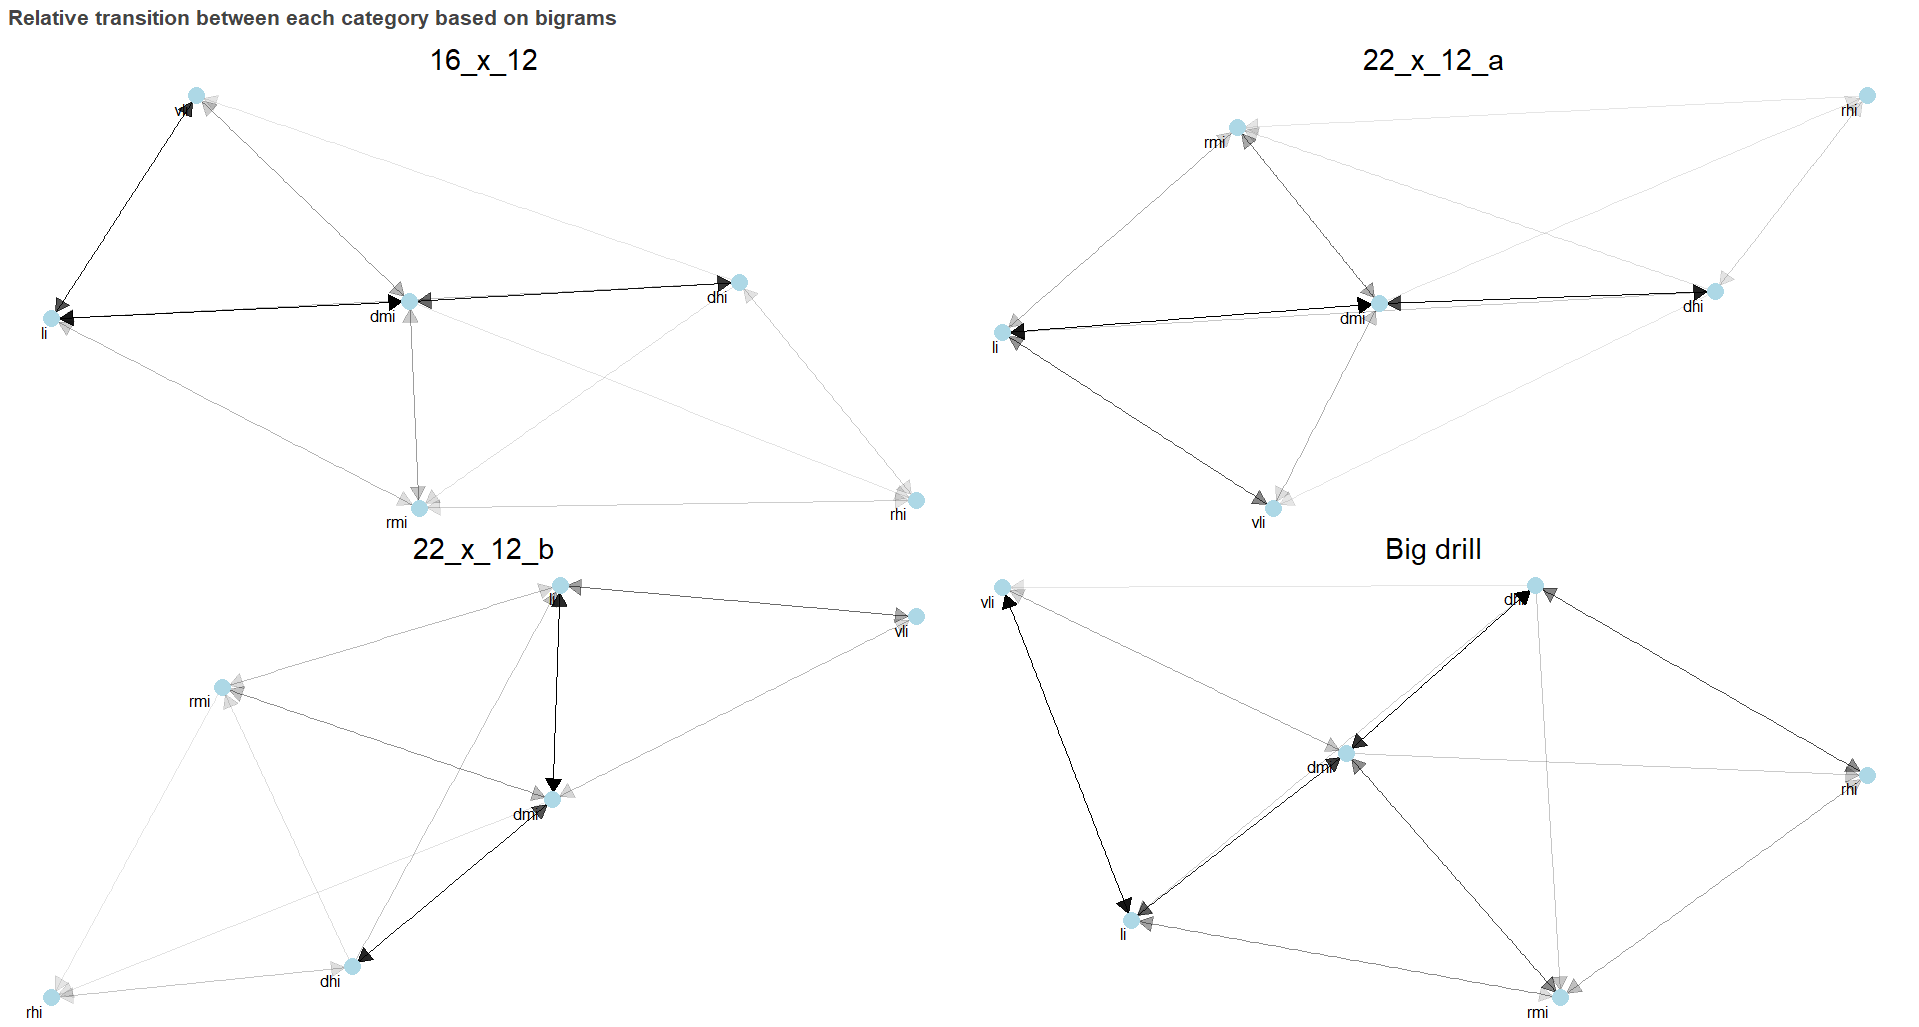
\includegraphics[width=1\linewidth]{img/networkPlot} 

}

\caption{Network plot illustrating the relative transition (the hue of the arrow) between the six FMP categories.}\label{fig:network}
\end{figure}

\end{document}
